%*****************************************
\chapter{A System}\label{ch:a_system}
%*****************************************

\section{Reflective Knowledge}

\begin{figure}[bth]
  \center
  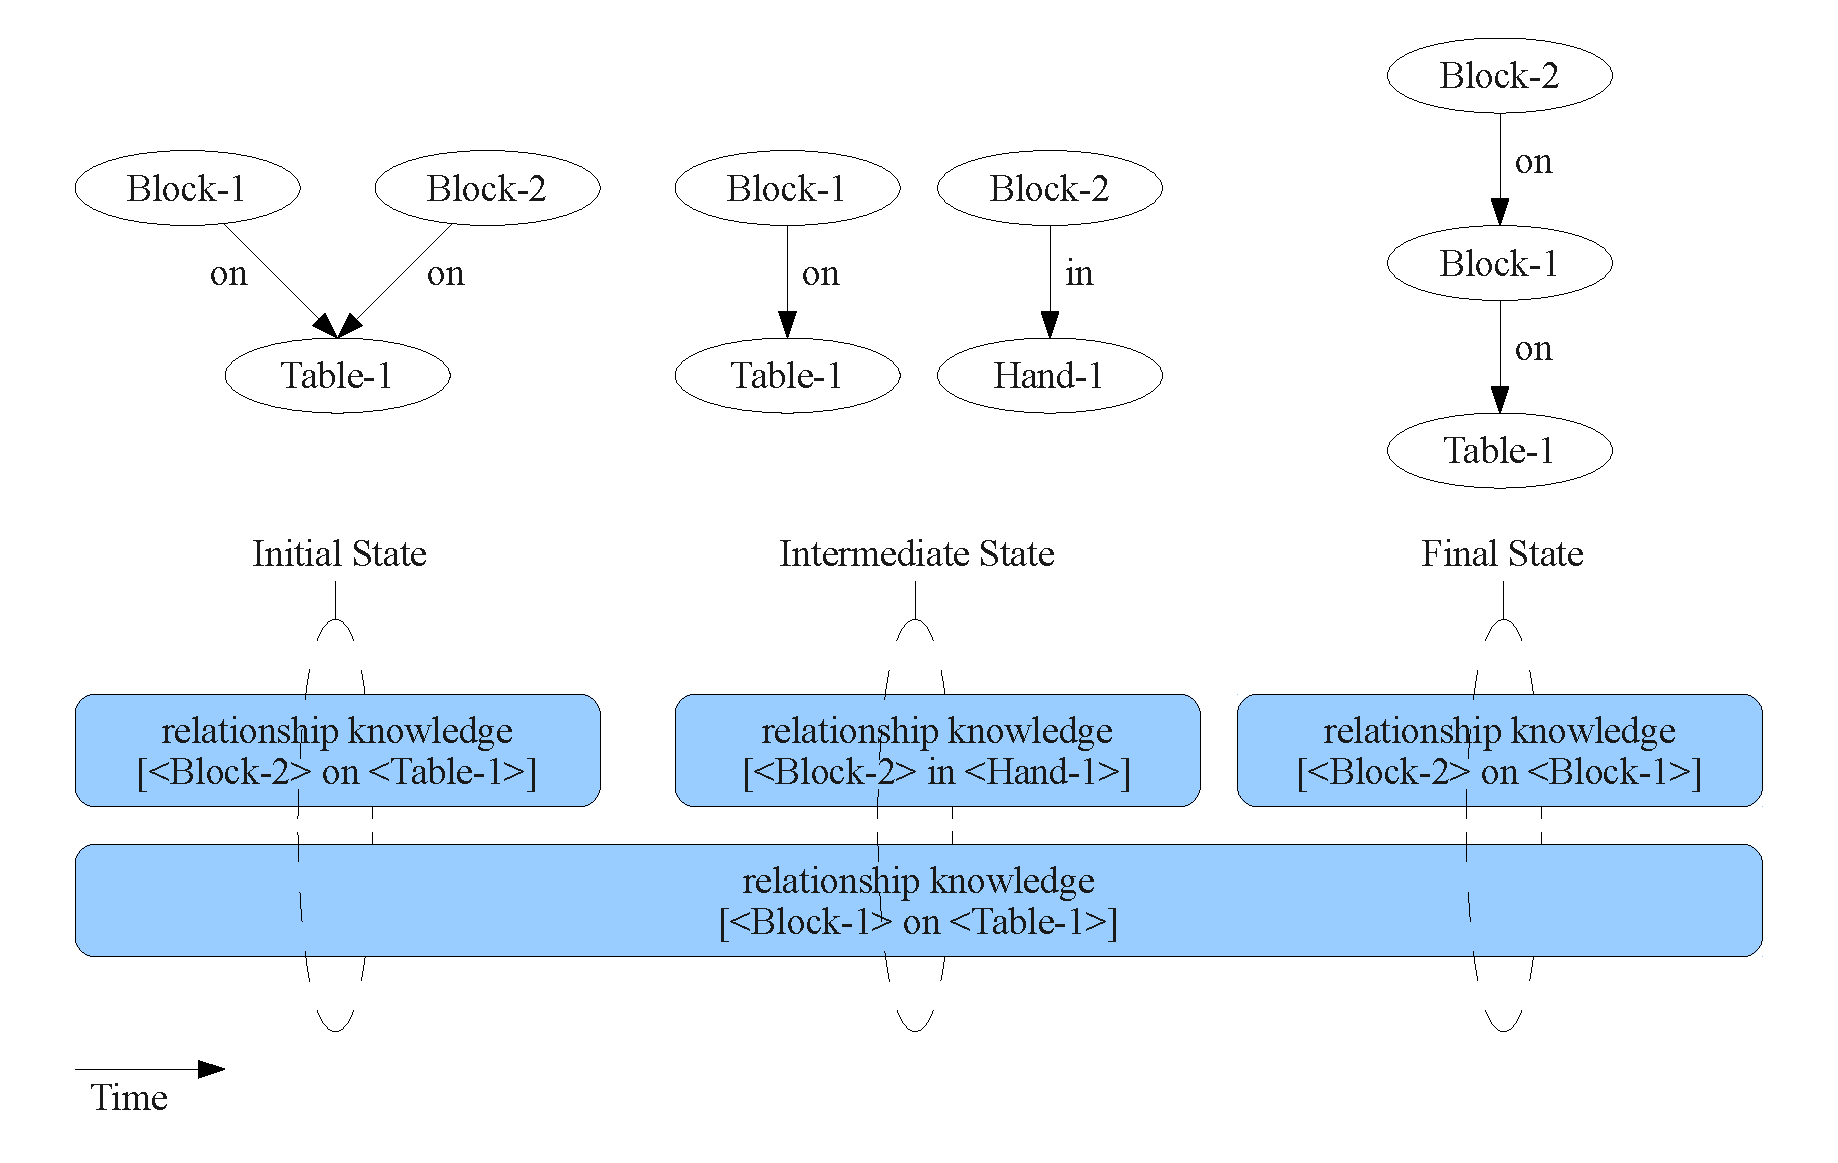
\includegraphics[width=12cm]{gfx/reflective_event_representation}
  \caption[A reflective event representation]{A reflective event representation shows the changes in a labeled graph.}
  \label{fig:reflective_event_representation}
\end{figure}


While the term meta-knowledge is used to describe the very general
idea of knowledge about knowledge, we use the term reflective
knowledge to refer to the specific type of meta-knowledge that refers
to knowledge about the changes to a knowledge structure.  If we keep
track of the changes to a knowledge structure, we can later integrate
these changes in order to obtain an equivalent form of that knowledge
structure as it was at any point in the past.


\section{Reflective Tracing}
\label{sec:reflective_tracing}

There are serious efficiency problems that must be carefully
sidestepped when one is dealing with reflective knowledge.  For
example, infinite reflection loops result in an infinite processor and
memory consumption pattern, after only a single change to a knowledge
representation.  The solution to this problem is to have various means
of controlling the reflective tracing focus.  We will discuss the
various methods for controlling the tracing focus of the reflective
memory that we have found useful in the development of our system in
Section~\ref{sec:methods_for_focusing_reflective_tracing}.


\section{Perceptual Support of Physical Knowledge}

\begin{figure}[bth]
  \center
  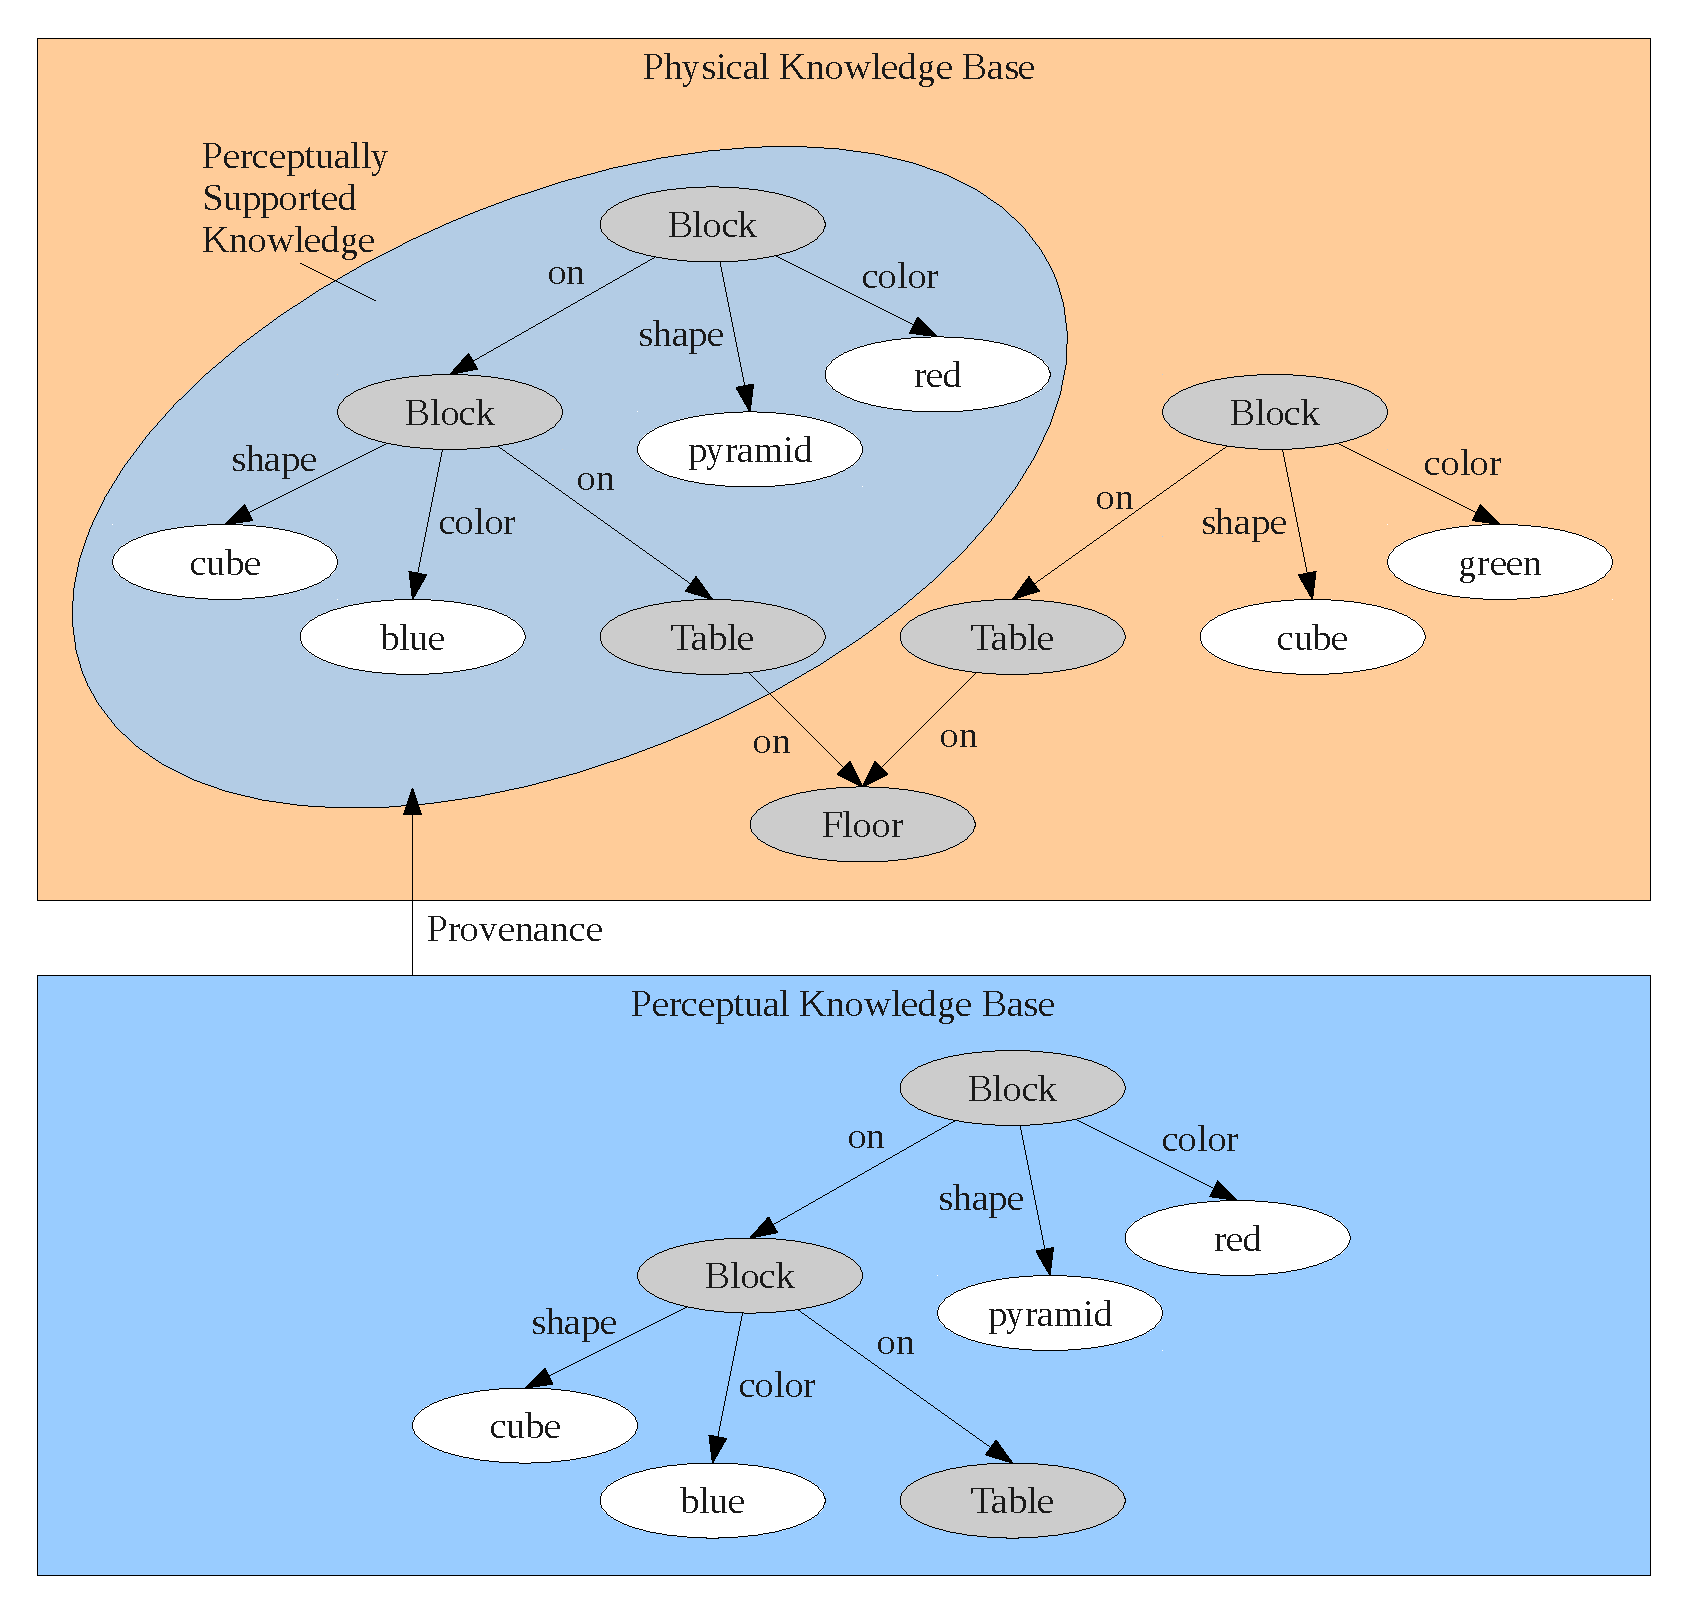
\includegraphics[width=10cm]{gfx/physical_perception}
  \caption[Perceptual provenance provides support for physical knowledge.]{Perceptual provenance provides support for physical knowledge.}
  \label{fig:physical_perception}
\end{figure}

See Figure~\ref{fig:physical_perception}.


\section{Debugging Plans by Reflectively Tracing the Provenance of Knowledge}

The thesis is focusing on provenance of knowledge.  From perception to
other knowledge representations, through planning and failed steps.
Normally, when plans fail, rule learning (or other learning method) is
used to update beginning and ending conditions for actions.  Very
complex planning methods exist that all assume that the current world
model is perfect (in either a deterministic or probabilistic
representation of the world).  Currently, plans are called policies
that handle all possible contingencies, in which the agent may find
itself.  When these plans fail, it is often unclear which part of the
plan was responsible for the failure.  In the simplest cases, a
specific low-level action may have been executing, which implies that
precondition categories were incorrectly mapped to postconditions or
the range of postconditions was not broad enough.  In the worst cases,
it is impossible to tell what part of the plan failed because the plan
is such a complicated tangle of compiled numbers that the only
recourse is to nudge a few of these numbers in a hill-climbing sense.
Rethinking this problem with my new approach that maintains provenance
for knowledge used in creating plans allows debugging the complex web
of knowledge and processes involved in creating that
knowledge---rather than simply updating the rules related to a single
action.

The planner that I've built in my system is not as complicated as
state of the art planners that currently exist in the field, but my
planner allows a reflective process to debug the failure of plans
created by our planner by tracing the provenance of the knowledge in
the plan representation itself.

\section{System Overview}

Building a machine that demonstrates the general intelligence required
for commonsense reasoning is a longstanding goal of the field of
artificial intelligence.  There have been many approaches to building
a machine that demonstrates general intelligence, some are based on
logical representations, others are based on large collections of
statistical knowledge, while still others approach the problem by
learning everything from scratch from the physical world.  We see the
problem as requiring a combination of many different types of
representations and reasoning processes.

We worked with Pushpinder Singh from 1999 to 2006 on the first version
of the Emotion Machine architecture, EM1 \citep{singh:2005}.  During
that period, we discussed that one weakness in the EM1 system is its
reliance on tracing only the declarative prolog statements, among
other necessary but untraced procedural code.  Although EM1 contained
a large amount of procedural knowledge, none of the effects of this
procedural knowledge could be debugged reflectively.  Toward solving
this problem, we have based our approach on a memory layer that can
trace the provenance of select memory events.

Because the Emotion Machine theory of mind requires a variety of many
reasoning processes to be controlled, we have built an operating
system on top of this traceable memory layer.

Further, the Emotion Machine is organized into layers of different
representations, so we have built a lisp-like language on top this
operating system.  The benefit of having a lisp-like language is the
language's ability to efficiently represent and simulate new
programming languages.

Within our lisp-like language we have written an implementation of a
layered reflective cognitive architecture, inspired by EM1.

Finally, we demonstrate our cognitive architecture in a rigid-body
physical environment, where multiple agents demonstrate learning from
both being told solutions to problems as well as learning from the
environment in which situations these solutions succeed or fail.  We
show how our procedurally traced memory can be used to assign credit
to those deliberative processes that are responsible for the failure,
facilitating learning how to better plan for these types of problems
in the future.

\section{Reflectively Traced Frame Memory}

Procedural tracing can be thought of as enabling a part of an
interpreter that checks for important events as a process runs.  This
ability can be used to trace the temporal order of events, i.e.
generating a trace, or to otherwise organize or summarize events in a
more useful way that can be used by other procedures, either
concurrently or after the fact.  Having this ability built into the
memory system, allows keeping track of the provenance of information as
it is written and read.  This ability is built into all structures in
the architecture, so if any tracing of data provenance is required at
any time for any object, this ability can be enabled.

At higher levels, these procedural tracing events result in event
streams that can be listened to by multiple concurrent processes that
each allocate iterators for a stream.  As a concurrent process
increments its iterator, it reasons about the event that has occurred in
the object memory, and the result of this reasoning is the creation of
meta knowledge in a causally consistent knowledge base.  This is an
example of the "glom" theory of cognitive evolution (reference needed; I
think you mentioned this in class), where cognitive abilities are added
on top of previous cognitive abilities without changing the underlying
functionality.  I've used procedural tracing to maintain multiple
consistent representations for the same knowledge.

When a plan fails, we need to correct the knowledge that generated that
plan.  When multiple processes are adding knowledge to the same
knowledge base, it becomes important to keep track of the provenance of
this knowledge, when we need to make distinctions between situations
that appear identical.  If we need to learn a new rule for
categorization of situations, or even a new category entirely, we need
to go back to the correct features and processes that performed those
categorizations of the identical situations that we need to further
distinguish.

\section{Methods for Focusing Reflective Tracing}
\label{sec:methods_for_focusing_reflective_tracing}
\marginpar{Section~\ref{sec:methods_for_focusing_reflective_tracing}
  is referenced from Section~\ref{sec:reflective_tracing}.}


\section{An Operating System}

We've written a multi-core operating system, including a
compiler, on top of this traceable and distributed memory layer.

Because the system is meant to combine many artificial intelligence
techniques, we have tested our platform running thousands of parallel
processes concurrently on an 8-core machine.  These processes can
control and watch one another execute.  We feel that the field of AI
is not separate from the low-level details of software engineering,
and my project embodies that philosophy.

Many people see AI as being a purely theoretical and mathematical
field, and we strongly disagree.  We need good software engineers in
order to solve most of the problems we face in getting these massive
software systems to work together.

\section{A Programming Language}

We have built a layered cognitive architecture on top of our custom
operating system, programming language, and compiler.

\subsection{Why not use Lisp?}

Lisp is a great programming language.  We wrote a custom programming
language for the project and didn't use lisp.  Lisp simply isn't fast
enough, and isn't very well supported; when you find a bug in a lisp
compiler, it is difficult to find the support to fix the bug.  We
wrote the first version of the reflectively traced memory system in
lisp and realized that Steele Bourne Common Lisp had memory bugs when
the system grew beyond 600 megabytes of RAM.  Allegro Lisp is a
commercial solution, but it costs many hundreds of dollars for their
commercial compiler, and we feel strongly against having that
commercial requirement for building academically intentioned
open-source software.  The main problem with lisp is it's lack of
speed and lack of support, so we found ourselves writing a lot of C
extensions even when programming in Lisp.  C is good for speeding up
inner loops of algorithms as well as necessary for interfacing with
the Linux, Mac, or Windows operating systems, which are all written in
C.

\section{A Layered Cognitive Architecture}

Further, we have developed a cognitive architecture within our
language that provides structures for layering reflective processes,
resulting in a hierarchy of control algorithms that respond to
failures in the layers below.




\section{Procedural Tracing}

The idea of having procedural tracing at the operating system level is
important because it does allow all programs running on the operating
system to assign credit to processes when bugs do occur.

%TS>> then you have to refer to the robust os literature and talk about their methods for
%TS>>tracing and justify it with their literature and then show how yours adds to it and 
%TS>>defend it against and in that community... ....might be a distraction .....
%TS>operating system... seems pretty general... how bout in the" memory's working set"

Although it is important to have protected memory boundaries between
programs for reasons of security, privacy, and stability, having good
ways for processes that do share memory to trace the provenance of
individual memory events, allows for much tighter and intelligent
interaction between all processes in the entire system.
        

\subsection{Trace Only an Appropriate Level of Abstraction}

It does not make sense to trace below a certain depth of processing.
If we were to trace all of the lowest level details of execution at
all times, there would be no way to take advantage of that amount
of detailed information.

There are barriers in my system for only allowing tracing to occur for
specific parts of the code.  The ability to focus the tracing of object
usage allows the possibility of tracing either high or low-level events
in a uniform manner.

\subsection{Keeping Tracing from Taking Too Much Time and Storage}

When a set of objects are out of the focus of tracing, these objects run
operate at full speed and do not increase the memory usage of the
tracing component.  There is a new proposal by McCarthy to build a new
programming language that remembers everything that it does; it is
called Elephant 2000 \citep{mccarthy:1994}.

